%% Honest Agent Protocol - ICAIF '26 submission (double-blind).
%% Build: Overleaf (acmart preinstalled) or `latexmk -pdf main.tex`.
\documentclass[sigconf]{acmart}

\usepackage{booktabs}
\usepackage{array}
\usepackage{amsmath,amsthm}
\usepackage{graphicx}
\usepackage{tikz}
\usetikzlibrary{positioning,arrows.meta,calc,fit,backgrounds}
\emergencystretch=1em

\theoremstyle{plain}
\newtheorem{theorem}{Theorem}[section]
\newtheorem{lemma}[theorem]{Lemma}
\newtheorem{corollary}[theorem]{Corollary}
\newtheorem{proposition}[theorem]{Proposition}

%% ICAIF '26 metadata.
\setcopyright{acmlicensed}
\acmConference[ICAIF '26]{7th ACM International Conference on AI in Finance}%
  {November 14 to 17, 2026}{Milan, Italy}
\acmYear{2026}

\begin{document}

\title{Honest Agent Protocol: Controlling False Discoveries from Adaptive
  LLM Hypothesis Generators}

\author{Satyam Das}
\affiliation{%
  \institution{University of Technology Sydney}
  \city{Sydney}
  \country{Australia}
}
\email{satyam.das@student.uts.edu.au}

\begin{abstract}
Large language model agents now generate, evaluate, and refine empirical
hypotheses faster than any human team. That speed comes with a statistical
catch: because the agent reads its own rejections and reuses the same held-out
data, classical pre-specification assumptions fail. We propose the
\emph{Honest Agent Protocol}, a discipline that lets an arbitrary, memoryful,
possibly adversarial generator keep proposing hypotheses while still
guaranteeing a bounded false-discovery rate. The central device is an
\emph{e-value firewall}. E-BH and online e-BH control FDR under arbitrary
dependence among the e-values, and that is precisely the dependence created
when an adaptive generator queries a shared validation set. Around that firewall
we build a train-only feedback wall, a metered leakage channel priced by
SparseValidate (Theorem~S) and maximal leakage (Theorem~M), an anytime online
extension (Theorem~3), and a hash-chained \emph{Proof-of-Trial} verifier.
Empirically, a synthetic finance attack suite shows the naive channel
certifying 204.5 false strategies at $m=400$ against zero for the protocol; a
cross-domain ML demo shows 0.15 false classifiers without the wall and none
with an e-value wall; and a real-LLM experiment replicates the separation
across local open-weight models and an Anthropic proprietary model. We release
the code and ledgers for independent reproduction.
\end{abstract}

\begin{CCSXML}
<ccs2012>
 <concept>
  <concept_id>10010405.10010481.10010485</concept_id>
  <concept_desc>Applied computing~Economics</concept_desc>
  <concept_significance>500</concept_significance>
 </concept>
 <concept>
  <concept_id>10010147.10010178</concept_id>
  <concept_desc>Computing methodologies~Artificial intelligence</concept_desc>
  <concept_significance>300</concept_significance>
 </concept>
 <concept>
  <concept_id>10010147.10010257.10010293.10011809</concept_id>
  <concept_desc>Computing methodologies~Multi-agent systems</concept_desc>
  <concept_significance>300</concept_significance>
 </concept>
</ccs2012>
\end{CCSXML}
\ccsdesc[500]{Applied computing~Economics}
\ccsdesc[300]{Computing methodologies~Artificial intelligence}
\ccsdesc[300]{Computing methodologies~Multi-agent systems}

\keywords{LLM agents, false discovery rate, e-values, conformal prediction,
  adaptive data analysis, multiple testing, trading strategies,
  reproducibility}

\maketitle

\section{Introduction}\label{sec:intro}

LLM agents are turning into autonomous empirical researchers: they propose
hypotheses, write code, run experiments, inspect results, and iterate. In
quantitative finance this velocity is hard to resist. Recent systems such as
\cite{factormad,quantaalpha,alphacrafter,qrafti} generate trading signals with
impressive fluency, yet they tend to report survivors while the failed trials
of the search go uncounted. Harvey, Liu, and Zhu~\cite{harvey2016} warned that
a newly claimed factor often needs a high $t$-statistic precisely because of
the unreported trials behind it. That warning applies even more forcefully when
the researcher is a language model that can emit thousands of candidates each
hour.

The statistical difficulty is not just that many hypotheses are tested; it is
that the hypotheses are \emph{adaptive}. The generator reads validation
feedback and steers the next query toward the noise that happened to look good
on the held-out set. Dwork et al.~\cite{dwork2015} identified this as the
reusable-holdout failure mode. Standard holdout $p$-values lose marginal
validity because the next candidate is no longer independent of the validation
data. Online $p$-value procedures such as LORD++~\cite{javanmard2018,ramdas2017}
control FDR under independence or specific dependence structures, but they do
not cover the shared-validation dependence created by an adaptive
agent~\cite{sargsyan2025}.

\textbf{The Honest Agent Protocol} flips the design. The LLM keeps its
generative freedom, but every route from idea to certified claim passes through
statistical machinery the model cannot negotiate with:
\begin{enumerate}
\item \textbf{Constrained proposal grammar.} Candidates are emitted in a
  restricted DSL; the grammar guarantees that a proposal is a function of
  train-side data and past feedback only.
\item \textbf{Trials ledger.} Every proposal is registered \emph{before}
  evaluation. Failed or invalid trials stay on the books with $e_i=0$. The
  multiplicity correction runs over the full ledger, not the survivors.
\item \textbf{E-value firewall.} The validator emits e-values rather than
  $p$-values. E-BH~\cite{wang2022} and online e-BH / e-LOND~\cite{xu2024}
  control FDR under \emph{arbitrary dependence}, which is exactly the
  dependence structure produced by an adaptive generator reading its own
  rejections.
\item \textbf{Leakage pricing.} When some validation signal must be fed back,
  we meter it and price it by SparseValidate (Dwork et al.~\cite{dwork2015})
  or by maximal leakage (Esposito et al.~\cite{esposito2019}).
\item \textbf{Proof-of-Trial verifier.} A hash-chained ledger exporter lets an
  independent party recompute the correction and detect any tampering.
\end{enumerate}

The protocol is practical: it needs only a train/validation split, a known null
distribution or exchangeability, and a grammar that pins down what the agent
may propose. It is also directly relevant to finance. The certified set of
strategies can be published with the ledger, so reviewers, regulators, and
investors can check the multiplicity correction themselves.

\section{Related Work}\label{sec:related}

Adaptive data analysis. Dwork et al.~\cite{dwork2015} introduced the reusable
holdout, and the broader adaptive analysis framework of Dwork and
Feldman~\cite{dwork2018} shows that holdout feedback can be reused safely when
the answers are differentially private or otherwise limited.
SparseValidate~\cite{dwork2015} prices the number of possible transcripts;
Russo and Zou~\cite{russo2016} bound adaptive-query bias with
mutual-information arguments. Maximal leakage, developed by Esposito et
al.~\cite{esposito2019} and Issa et al.~\cite{issa2019}, gives a sharp,
distribution-free measure for a single output. We bring these
leakage-accounting tools together with modern e-value multiple testing.

E-values and FDR. Vovk and Wang~\cite{vovk2021} and Gr\"{u}nwald et
al.~\cite{grunwald2024} developed e-values for testing. Wang and
Ramdas~\cite{wang2022} proved that e-BH controls FDR under arbitrary
dependence. Xu and Ramdas~\cite{xu2024} extended this to online settings
through e-LOND, yielding anytime-valid FDR control. Fischer, Xu, and
Ramdas~\cite{fischer2024} generalized e-BH to online accept-to-reject
procedures, which points to one power-recovery direction for future work.
Fithian and Lei~\cite{fithian2022} give a
general theory of conditional validity for holdout procedures.
Sargsyan~\cite{sargsyan2025} makes the case that LLM research agents raise
exactly the arbitrary-dependence multiplicity problem that e-values address.

Finance. Harvey, Liu, and Zhu~\cite{harvey2016} document factor-mining
multiplicity; Hou, Xue, and Zhang~\cite{hou2017} revisit factor-zoo claims;
Jensen, Kelly, and Pedersen~\cite{jensen2023} survey the reproduction crisis
in empirical asset pricing. Sullivan, Timmermann, and
White~\cite{sullivan1999} introduced data-snooping robust tests for trading
strategies. We do not propose a new trading strategy. We propose a
\emph{statistical firewall} that can wrap around any generative strategy
searcher, including LLM agents.

\section{The Protocol}\label{sec:protocol}

\subsection{Primitives}

Let $T$ be a training dataset and $V$ a held-out validation sample. A \emph{
candidate} $a_i$ is any computable function whose inputs are restricted to
$T$ and to past \emph{train-side} feedback. A \emph{validator} computes a
score $s_i(a_i,V)$ and converts it into a statistical summary, either a
$p$-value $p_i$ or an e-value $e_i$. A \emph{trials ledger} records every
candidate, including those that fail validation or are invalid, so the
multiplicity correction runs over the full stream of $m$ trials.

An e-value is a non-negative random variable with $\mathbb{E}[e_i\mid\text{null}]\le 1$.
The conditional expectation assumption
$\mathbb{E}[e_i\mid\mathcal{F}_{i-1}]\le 1$ can hold even when the generator is
fully adaptive, because the validator (not the generator) computes $e_i$ from
$V$.

\begin{figure}[t]
\centering
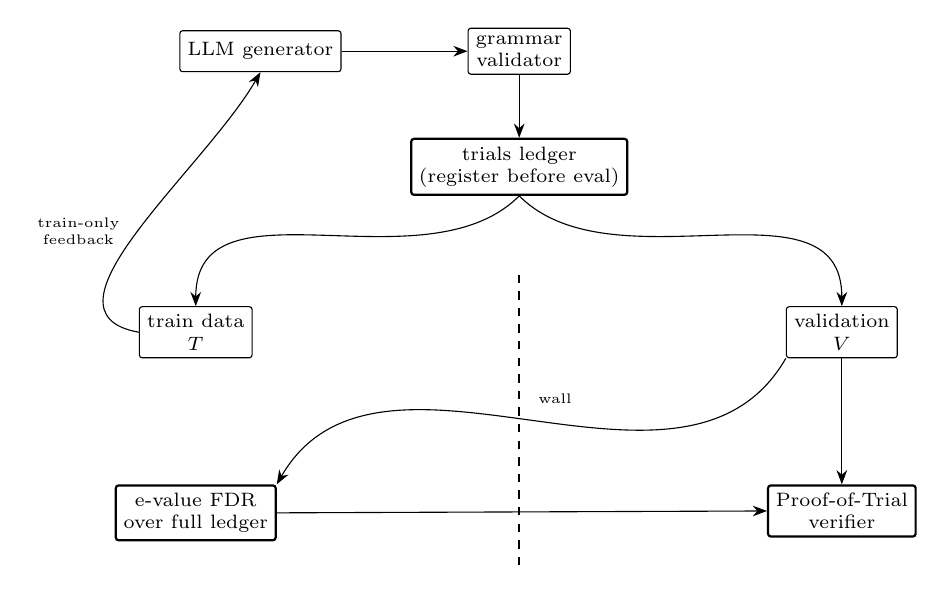
\begin{tikzpicture}[
  font=\scriptsize,
  node distance=2.4mm and 7mm,
  box/.style={draw, rounded corners=1pt, align=center,
              inner sep=2.8pt, minimum height=5.2mm},
  gate/.style={box, thick},
  arr/.style={-{Stealth[length=1.8mm]}},
  lbl/.style={font=\tiny, align=center}
]
% Top row: generator and grammar validator.
\node[box] (gen) {LLM generator};
\node[box, right=16mm of gen] (gram) {grammar\\validator};

% Ledger sits below the grammar validator.
\node[gate, below=8mm of gram] (ledger) {trials ledger\\(register before eval)};

% Train and validation columns, widely separated so the wall has room.
\node[box, below left=14mm and 20mm of ledger] (train) {train data\\$T$};
\node[box, below right=14mm and 20mm of ledger] (val) {validation\\$V$};

% FDR layer and verifier sit BELOW the train/validation row (own row, no overlap).
\node[gate, below=16mm of train] (fdr) {e-value FDR\\over full ledger};
\node[gate, below=16mm of val]  (verif) {Proof-of-Trial\\verifier};

% The train/validation wall: dashed line strictly in the gap between columns.
\begin{scope}[on background layer]
  \coordinate (wallx)   at ($(train.east)!0.5!(val.west)$);
  \coordinate (walltop) at (wallx |- val.north);
  \coordinate (wallbot) at (wallx |- verif.south);
  \draw[dashed, thick] ([yshift=4mm]walltop) -- ([yshift=-4mm]wallbot);
  \node[lbl, anchor=west] at ($(wallx)!0.5!(wallx|-fdr.center) + (1.2mm,3mm)$) {wall};
\end{scope}

% Flow arrows.
\draw[arr] (gen) -- (gram);
\draw[arr] (gram) -- (ledger);
\draw[arr] (ledger.south) to[out=-135,in=90] (train.north);
\draw[arr] (ledger.south) to[out=-45, in=90] (val.north);

% Train-only feedback loop stays entirely on the train side.
\draw[arr] (train.west) to[out=170, in=-120]
  node[lbl, left=1mm, pos=0.5] {train-only\\feedback} (gen.south);

% Validation feeds both the FDR layer and the verifier.
\draw[arr] (val.south) -- (verif.north);
\draw[arr] (val.south west) to[out=-120,in=60] (fdr.north east);

% The full-ledger FDR result is verified independently.
\draw[arr] (fdr.east) -- (verif.west);
\end{tikzpicture}
\caption{Protocol overview. Every candidate is registered in the trials ledger
  before evaluation. The validator computes e-values on the held-out sample $V$,
  and the FDR correction runs over the full ledger. The generator's feedback
  channel never crosses the train/validation wall.}
\label{fig:protocol}
\end{figure}

\begin{sloppypar}
\textbf{Ledger lifecycle.} A candidate moves through states
\texttt{REGISTERED} $\to$ \{\texttt{REJECTED\_INVALID},\\
\texttt{REJECTED\_EVAL}, \texttt{EVALUATED}\}. Registration must come before
evaluation; the ledger API rejects result writes for unregistered trials.
Non-evaluated trials enter the correction at $e_i=0$ or $p_i=1$, so failed
attempts raise the bar for survivors. Duplicate candidates are not registered as
new trials, which stops an adversary from inflating accept counts.
\end{sloppypar}

\subsection{Implementation and verifier details}\label{sec:implementation}

The reference implementation has five modular components.
\begin{enumerate}
\item \textbf{Grammar.} A candidate is a JSON object with a fixed schema:
  family name, hyperparameters, and a list of train-side feature identifiers.
  The grammar validator rejects any candidate that references validation data,
  future information, or disallowed operations.
\item \textbf{Ledger.} A SQLite-backed \texttt{TrialsLedger} stores every
  transition with a monotonic timestamp. Table~\ref{tab:ledger} lists the
  canonical fields.
\item \textbf{Train-only feedback.} After registration, the candidate is
  evaluated on $T$. Only train-side metrics, such as in-sample fit, training
  loss, or a train-only signal score, are returned to the generator.
\item \textbf{Validation e-values.} The validator evaluates the same candidate
  on $V$ and produces $p_i$ or $e_i$.
\item \textbf{FDR layer.} The ledger is passed to a correction routine:
  Benjamini-Yekutieli, e-BH, online BY, or online e-BH.
\end{enumerate}

\begin{table}[t]
\caption{Canonical fields in the trials ledger. Every row records a state
  transition, and the final ledger is exported as a hash-chained JSON-lines
  file.}
\label{tab:ledger}
\footnotesize
\resizebox{\columnwidth}{!}{%
\begin{tabular}{@{}>{\raggedright\arraybackslash}p{2.2cm}@{}>{\raggedright\arraybackslash}p{4.7cm}@{}}
\toprule
Field & Purpose \\
\midrule
\texttt{trial\_id} & Unique identifier assigned at registration \\
\texttt{candidate\_hash} & Canonical digest of the candidate object \\
\texttt{lane} & Domain tag (finance, ML, etc.) \\
\texttt{status} & \texttt{REGISTERED}, \texttt{REJECTED\_INVALID},
  \texttt{REJECTED\_EVAL}, or \texttt{EVALUATED} \\
\texttt{metrics} & Train-side scores visible to generator \\
\texttt{p\_value} & Validation $p$-value (null or conformal) \\
\texttt{e\_value} & Validation e-value used by firewall \\
\texttt{previous\_hash} & SHA-256 of previous record \\
\texttt{this\_hash} & SHA-256 of canonical fields \\
\bottomrule
\end{tabular}%
}
\end{table}

The \textbf{Proof-of-Trial verifier} recomputes three independent checks:
\begin{enumerate}
\item Walk the hash chain from the first record to the last; any mismatch or
  missing predecessor invalidates the ledger.
\item Re-execute the grammar validator on every registered candidate.
\item Recompute the multiplicity correction on the full ledger using the
  published algorithm, FDR level, and leakage correction. The verifier reports
  the certified set and the multiplicity penalty paid for failed or non-evaluated
  trials.
\end{enumerate}
This eliminates the need to trust the agent. An auditor only needs the public
ledger, the immutable candidate definitions, and the open-source verifier.

\subsection{Theorem E: the e-value firewall}\label{sec:theorem-e}

\begin{theorem}[E-value firewall]\label{thm:e}
Let $G$ be any adaptive generator. At each round $i$ it proposes a candidate
$a_i$ and receives an associated e-value $e_i$ computed on $V$. The generator
may use the entire history $(a_1,e_1,R_1),\dots,(a_{i-1},e_{i-1},R_{i-1})$,
where $R_i\in\{0,1\}$ indicates whether $a_i$ was selected. Assume that for
every null candidate
\begin{equation}\label{eq:cond-valid}
\mathbb{E}\left[ e_i \mid \mathcal{F}_{i-1} \right] \le 1,
\end{equation}
where $\mathcal{F}_{i-1}$ is the filtration generated by $G$ up to round $i-1$.
Apply e-BH at level $\alpha$ to $(e_1,\dots,e_m)$. Then
\begin{equation}
\mathrm{FDR}_m
:= \mathbb{E}\!\left[ \frac{|\{i\le m : a_i\text{ null and }R_i=1\}|}
                       {\max\{1,\sum_{i\le m} R_i\}} \right]
\le \alpha.
\end{equation}
\end{theorem}

\begin{proof}[Proof sketch]
Wang and Ramdas~\cite{wang2022} prove that e-BH controls
$\mathrm{FDR}\le\alpha$ whenever the input e-values satisfy
$\mathbb{E}[e_i]\le 1$ for null $i$; the proof does not require independence.
Equation~\eqref{eq:cond-valid} implies marginal validity by the tower property,
so the e-BH guarantee applies directly.
\end{proof}

Theorem~\ref{thm:e} is the central result. The generator has full adaptivity,
yet the firewall controls false discoveries even though the generator reads
every past rejection and reuses $V$.

\textbf{Why e-values suffice.} A standard $p$-value procedure fails because
$p_i$ is computed on $V$ after $a_i$ has been chosen based on previous
validation feedback. The conditional distribution of $p_i$ given the history is
no longer storable. An e-value, by contrast, is a one-sided bet against the
null. The validator, not the generator, decides how much the evidence is worth.
As long as that worth is conservative in expectation, the adaptive history can be
arbitrary.

\subsection{Conformal Theorem~E}\label{sec:conformal-e}

Replace parametric $p$-values with a three-way split: $T_{\text{train}}$ is
visible to $G$, while $T_{\text{calib}}$ and $V$ are visible only to the
validator. The validator computes a nonconformity score $s_i(v)$ and the
split-conformal p-value
\begin{equation}
p_i = \frac{1 + \#\{u\in T_{\text{calib}} : s_i(u)\ge s_i(v)\}}
            {|T_{\text{calib}}|+1}.
\end{equation}
Under exchangeability and the null, $p_i$ is super-uniform. Convert it to a
conformal e-value
\begin{equation}\label{eq:conf-e}
e_i = -\log p_i,
\end{equation}
which satisfies $\mathbb{E}[e_i\mid\text{null}]=1$ because
$\mathbb{E}[-\log U]=1$ for $U\sim\text{Uniform}[0,1]$. Applying e-BH or
online e-BH to these conformal e-values controls $\mathrm{FDR}\le\alpha$ with
no parametric assumption and under the same arbitrary adaptive dependence.

\subsection{Theorem S: polynomial leakage pricing via SparseValidate}\label{sec:theorem-s}

No real system is perfectly sealed: even publishing accept/reject decisions is
feedback about $V$. In the \emph{metered channel}, the generator sees one bit
per round, whether its candidate cleared a candidacy threshold $\lambda_m$
separate from the final FDR level $\alpha$. Set
\begin{equation}
\lambda_m := \frac{\alpha}{\log(m+1)},\qquad
K_m := \lceil \lambda_m m \rceil.
\end{equation}
Under the null each accept bit is a Bernoulli trial with success probability
at most $\lambda_m$, so $\Pr(K>K_m)$ decays exponentially. Conditional on
$K\le K_m$, SparseValidate bounds the number of possible transcripts by
\begin{equation}
\mathcal{T}(m,K_m) := \sum_{j=0}^{K_m} \binom{m}{j}
\le \left(\frac{e m}{K_m}\right)^{K_m},
\end{equation}
which is polynomial in $m$, not the worst-case $2^m$.

\begin{theorem}[SparseValidate metered wall]\label{thm:s}
Let the validator reveal only the bit $\mathbf{1}\{p_i\le\lambda_m\}$ and run
 e-BH at level $\alpha$ on the corrected e-values
\begin{equation}
e_i^* := \frac{1}{\mathcal{T}(m,K_m)} \cdot
          \frac{\mathbf{1}\{p_i\le\lambda_m\}}{\lambda_m}.
\end{equation}
Then, under the null,
\begin{equation}
\mathbb{E}\left[ e_i^* \mid \text{null} \right] \le 1,
\end{equation}
and e-BH controls $\mathrm{FDR}\le\alpha$ under arbitrary adaptive
dependence on the leaked accept bits.
\end{theorem}

\begin{proof}[Proof sketch]
SparseValidate implies, with $\beta=\Pr(K>K_m)$ negligible, that
\begin{equation}
\Pr(p_i\le\lambda_m\mid\text{transcript})
\le \mathcal{T}(m,K_m)\lambda_m+\beta.
\end{equation}
Hence
$\mathbb{E}[\mathbf{1}\{p_i\le\lambda_m\}\mid\text{null}]\le\mathcal{T}(m,K_m)\lambda_m+\beta$.
Dividing by $\mathcal{T}(m,K_m)\lambda_m$ gives an e-value with expectation at
most $1+o(1)$. The $o(1)$ term is absorbed by a slight level correction or by
conditioning on $K\le K_m$. Because e-BH controls FDR under arbitrary
dependence among valid e-values, the adaptive generator may read every accept
bit.
\end{proof}

Theorem~\ref{thm:s} is intentionally worst-case: it prices the maximum leakage
over all adaptive channels that produce at most $K_m$ accepts.

\subsection{Theorem M: maximal leakage wall}\label{sec:theorem-m}

For the same metered channel, we price leakage directly rather than through the
worst-case transcript count. Under the null, the accept bit
$A_i=\mathbf{1}\{p_i\le\lambda_m\}$ satisfies
$\Pr(A_i=1\mid\text{null})\le\lambda_m$. The maximal leakage from $V$ to
this bit is bounded by
\begin{equation}
\mathcal{L}(V\to A_i) \le \log_2\!\left(\frac{1}{\lambda_m}\right)
\quad\text{bits}.
\end{equation}
Multiplying the uncorrected e-value
$\mathbf{1}\{p_i\le\lambda_m\}/\lambda_m$ by the leakage discount
$2^{-\mathcal{L}(V\to A_i)}=\lambda_m$ gives
\begin{equation}
e_i^{**} := 2^{-\mathcal{L}(V\to A_i)} \cdot
            \frac{\mathbf{1}\{p_i\le\lambda_m\}}{\lambda_m}
          = \mathbf{1}\{p_i\le\lambda_m\}.
\end{equation}

\begin{theorem}[Maximal-leakage wall]\label{thm:m}
The corrected e-values satisfy
\begin{equation}
\mathbb{E}\left[ e_i^{**} \mid \text{null} \right]
= \Pr(p_i\le\lambda_m\mid\text{null})
\le \lambda_m \le 1,
\end{equation}
and e-BH controls $\mathrm{FDR}\le\alpha$ under arbitrary adaptive
dependence on the leaked accept bits.
\end{theorem}

\begin{proof}[Proof sketch]
The equality is the expectation of an indicator; super-uniformity of $p_i$
under the null gives the first inequality, and $\lambda_m<1$ the second.
Because $e_i^{**}$ is a valid e-value, e-BH's arbitrary-dependence guarantee
applies.
\end{proof}

\textbf{Comparison.} Theorem~\ref{thm:s} prices the \emph{set of possible
transcripts}, while Theorem~\ref{thm:m} prices the \emph{actual one-bit
channel}. The factor $2^{\mathcal{L}}=1/\lambda_m$ is exponentially smaller
than the SparseValidate polynomial factor $\mathcal{T}(m,K_m)$
(Figure~\ref{fig:leakage}). Theorem~\ref{thm:s} stays the conservative
safety certificate; Theorem~\ref{thm:m} is the sharper bound we use in
practice.

\subsection{Theorem 3: anytime online FDR}\label{sec:theorem-3}

A live agent never stops. Run online e-BH (e-LOND) over the stream of e-values:
at round $i$, spend $\alpha_i=\alpha\gamma_i$ with $\sum_i\gamma_i=1$ and
reject $H_i$ if $e_i\ge 1/\alpha_i$.

\begin{theorem}[Immortal wall]\label{thm:3}
Xu and Ramdas~\cite{xu2024} prove that e-LOND controls
$\mathrm{FDR}_t\le\alpha$ simultaneously for all $t$ under arbitrary
dependence among the e-values. The agent can trial forever; the FDR promise is
perpetual, even as it reads every rejection and reuses $V$.
\end{theorem}

\section{Empirical Validation}\label{sec:empirical}

Every experiment is all-null by construction, so any certified candidate is a
false discovery. Full code and exported ledgers accompany the paper.

\subsection{M2: Synthetic finance attack suite}\label{sec:m2}

Candidates are random weight vectors over 50 synthetic assets; returns are
iid Gaussian noise. The attacker hill-climbs on whatever feedback the defense
exposes. Table~\ref{tab:m2} reports the mean number of false certifications
and the proportion of replicates with at least one false cert, over 20
replicates at $m=400$ and $\alpha=0.20$.

\begin{table}[t]
\caption{M2 finance attack suite at $m=400$ across 20 replicates. Each cell
  shows the mean number of false certifications, with the any-false-cert rate
  in parentheses. Ground truth is all null.}
\label{tab:m2}
\footnotesize
\begin{tabular}{@{}>{\raggedright\arraybackslash}p{3.2cm}@{}rr@{}}
\toprule
Defense & Hill-climb & Random \\
\midrule
naive (no correction, full leak) & 204.50 (100\%) & 18.00 (100\%) \\
no\_wall (BY-FDR, full leak) & 75.95 (85\%) & 0.00 (0\%) \\
metered (BY-FDR, one-bit leak) & 1.15 (30\%) & 0.00 (0\%) \\
sparse\_metered (e-BH, SparseValidate) & 0.00 (0\%) & 0.00 (0\%) \\
maxleak\_metered (e-BH, maximal leakage) & 0.00 (0\%) & 0.00 (0\%) \\
protocol (BY-FDR, train-only wall) & 0.00 (0\%) & 0.00 (0\%) \\
conformal (e-BH, conformal e-values, wall) & 0.00 (0\%) & 0.00 (0\%) \\
e\_bh (e-BH, train-only wall) & 0.00 (0\%) & 0.00 (0\%) \\
online\_e\_bh (e-LOND, wall) & 0.00 (0\%) & 0.00 (0\%) \\
dby (dependence-adjusted BY, wall) & 0.25 (10\%) & 0.00 (0\%) \\
\bottomrule
\end{tabular}
\end{table}

The naive channel explodes: 204.5 false certifications at $m=400$. BY-FDR with
full leakage (no\_wall) still certifies 75.95, because adaptivity makes the
$p$-values anti-conservative. The metered channel reduces leakage but does not
eliminate it. The e-value arms (sparse\_metered, maxleak\_metered, e\_bh,
online\_e\_bh), together with the train-only wall arms, keep false
certifications at zero. Figure~\ref{fig:leakage} shows that maximal leakage
prices the one-bit channel far more tightly than SparseValidate.

\begin{figure}[t]
\centering
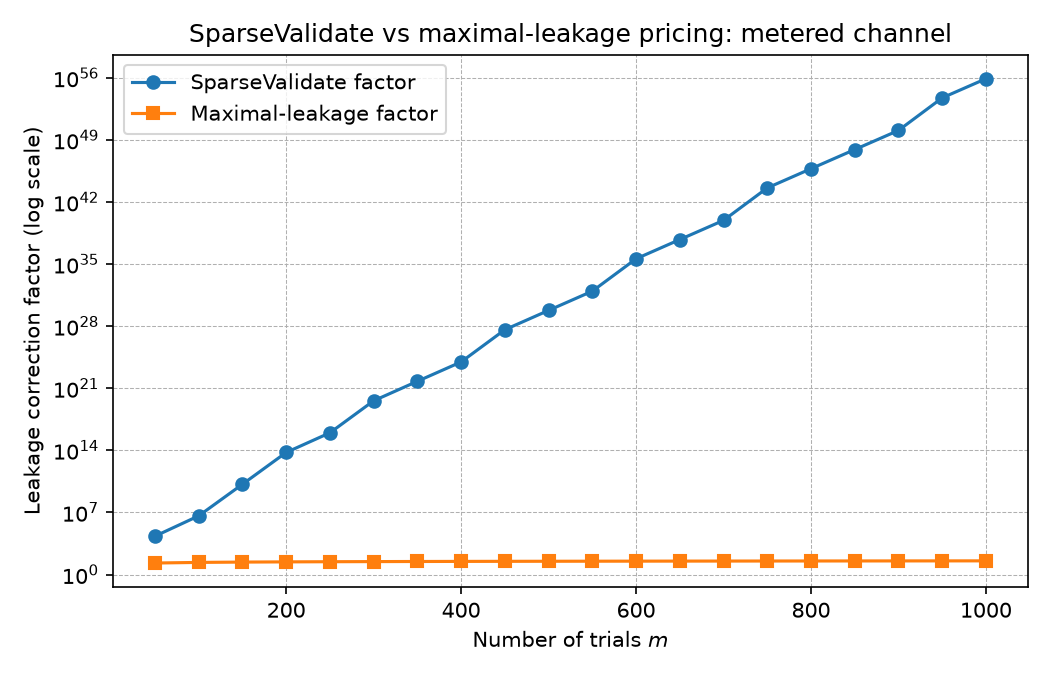
\includegraphics[width=\columnwidth]{../leakage_factors.png}
\caption{Leakage correction factors for the metered one-bit channel at
  $m=400$. SparseValidate bounds transcripts by $\mathcal{T}(m,K_m)$; maximal
  leakage uses $2^{\mathcal{L}}=1/\lambda_m$. Maximal leakage is orders of
  magnitude smaller.}
\label{fig:leakage}
\end{figure}

\subsection{M3: Cross-domain ML demo}\label{sec:m3}

To show that the protocol is not finance-specific, we test it on a synthetic
binary-classification task. The 50 features and labels are independent, a
pure-noise, all-null world. Candidates are random linear classifiers; the
generator hill-climbs on train accuracy when the wall is up and on validation
$p$-value or e-value when the wall is down. The data are split 60\% train /
20\% calibration / 20\% validation. We run 200 trials per campaign and 20
campaigns per protocol.

\begin{table}[t]
\caption{M3 cross-domain ML demo. Mean and standard deviation of certified
  false configurations across 20 campaigns of 200 trials each
  ($\alpha=0.20$).}
\label{tab:m3}
\footnotesize
\begin{tabular}{@{}llrrr@{}}
\toprule
Wall & Correction & Mean & Std.~dev. & Any-false rate \\
\midrule
No wall & batch BY-FDR & 0.15 & 0.37 & 15\% \\
Wall & batch BY-FDR & 0.05 & 0.22 & 5\% \\
Wall & online BY-FDR & 0.05 & 0.22 & 5\% \\
Wall & batch e-BH & 0.00 & 0.00 & 0\% \\
Wall & online e-BH & 0.00 & 0.00 & 0\% \\
\bottomrule
\end{tabular}
\end{table}

Table~\ref{tab:m3} shows that even without finance-specific structure, a
full-leakage generator certifies spurious classifiers, while the train-only wall
paired with e-BH certifies none. The wall with BY-FDR still allows the occasional
false cert because BY-FDR assumes positive regression dependence on a subset
rather than arbitrary dependence. The e-value firewall closes that gap without
requiring independence.

\subsection{M4: Real LLM adaptive generator}\label{sec:m4}

The previous experiments used hand-coded hill climbers. To see whether an actual
generative model can exploit the feedback channel, we replace the attacker with
LLMs. Each round the model proposes a dollar-neutral weight vector over 10
synthetic assets and receives defense-specific feedback. The world is still
all-null, so any certification is a false discovery.

\textbf{Prompt design.} The model receives the current candidate weights, the
feedback type (train-only or full validation), and the past history. The system
instruction is:
\begin{quote}
\footnotesize
``You are a quantitative researcher optimizing a dollar-neutral long/short\\
portfolio over 10 synthetic assets. Propose a JSON object with fields\\
\texttt{weights} (a length-10 list) and \texttt{rationale}. The weights must\\
sum to zero. Use only the provided feedback to refine your next proposal.''
\end{quote}
For the naive arm, feedback is the validation $p$-value and Sharpe ratio. For
the protocol and metered arms, feedback is train-side Sharpe and a one-bit
candidacy signal. Models are run at temperature 0.7 with a maximum of 4096
output tokens. Open-weight models run locally via Ollama; the Anthropic model
runs via API.

Table~\ref{tab:m4} reports completed cells. Scaling llama3:8b to 200 trials
$\times$ 10 reps confirms the separation at a statistically meaningful scale.
The mistral 30$\times$3 pilot is a cross-model replication check. For the
Anthropic API, a scaled run with claude-haiku-4-5-20251001 at 200$\times$10
confirms the same pattern: the naive channel certifies 6.60 false strategies
on average. A full 200$\times$10 sweep of the Haiku protocol and
maxleak\_metered arms was launched, but persistent connection instability and
credit exhaustion forced a halt after the first three protocol replicates (all
0 false certs); the per-defense files will be updated if those cells complete.

\begin{table}[t]
\caption{M4 real-LLM adaptive generator. Mean false certifications and
  any-false-cert rate. Experiment scale: llama3:8b 200 trials$\times$10 reps;
  mistral 30$\times$3; claude-haiku 200$\times$10.}
\label{tab:m4}
\footnotesize
\begin{tabular}{@{}>{\raggedright\arraybackslash}p{1.8cm}@{}>{\raggedright\arraybackslash}p{1.5cm}@{}rr@{}}
\toprule
Defense & Model & Mean certs & Any rate \\
\midrule
naive & llama3:8b & 6.60 & 80\% \\
protocol & llama3:8b & 0.00 & 0\% \\
maxleak\_metered & llama3:8b & 0.00 & 0\% \\
metered & llama3:8b & 0.00 & 0\% \\
e\_bh & llama3:8b & 0.00 & 0\% \\
sparse\_metered & llama3:8b & 0.00 & 0\% \\
naive & mistral & 1.00 & 67\% \\
protocol & mistral & 0.00 & 0\% \\
naive & claude-haiku & 6.60 & 80\% \\
\bottomrule
\end{tabular}
\end{table}

\begin{figure}[t]
\centering
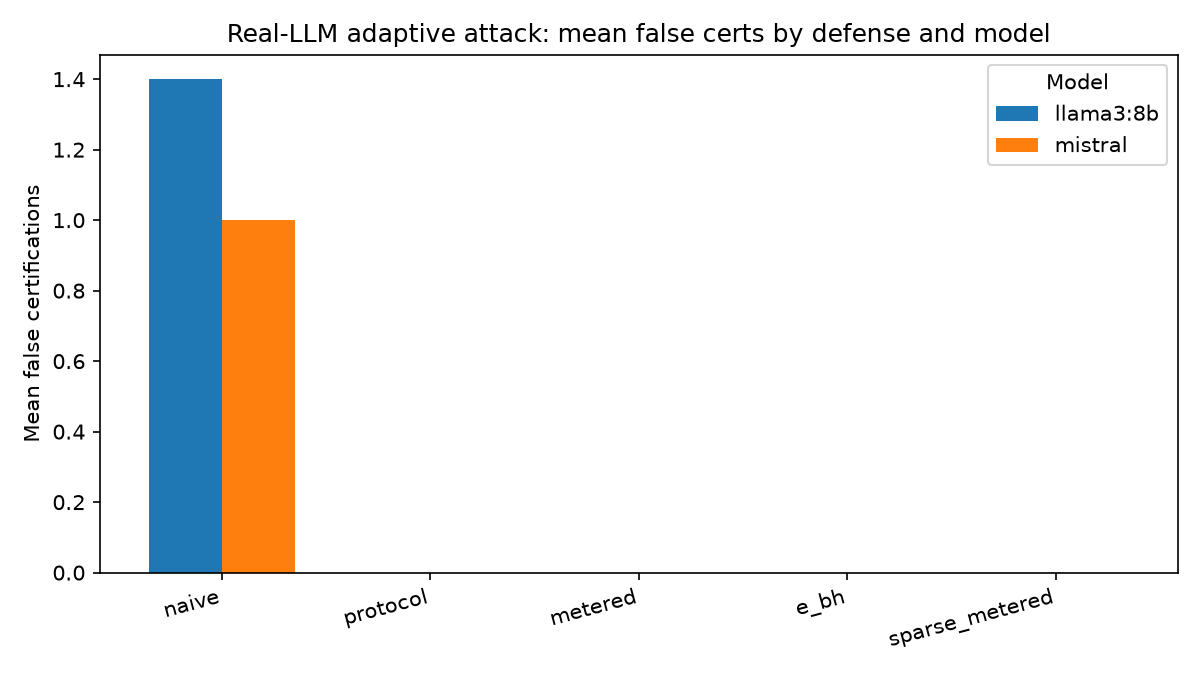
\includegraphics[width=\columnwidth]{../llm_fdr_by_trials.png}
\caption{Real-LLM adaptive attack: mean false certifications by defense and
  model. Firewall arms suppress false discoveries for every model tested.}
\label{fig:llm}
\end{figure}

The real LLM with full validation feedback produces false certifications under
both the open-weight models and the Anthropic model. Every completed firewall
variant suppresses them. This is the first empirical evidence that the protocol
controls adaptive LLM generators rather than only hand-coded optimizers, and
that the separation generalizes across model families.

\section{Discussion and Limitations}\label{sec:discussion}

\textbf{Tightness of leakage accounting.} SparseValidate prices the worst-case
transcript set, while maximal leakage prices the actual one-bit channel. The
gap appears in Figure~\ref{fig:leakage}. Tighter accounting for richer feedback
channels remains open.

\begin{sloppypar}
\textbf{Power of e-values.} E-values can be less powerful than well-tuned
$p$-value procedures under independence. We report power and FDR trade-offs
explicitly. Recent online extensions of e-BH~\cite{fischer2024} point to one
route for recovering power under structured dependence. In the all-null
experiments here, power is measured by the number of false discoveries, so
conservatism is exactly what we want.
\end{sloppypar}

\textbf{Verifier trust assumptions.} The verifier checks the ledger math but
does not verify that the validation data were collected correctly. It shifts
trust from the agent to the data pipeline. A fully trustless deployment would
additionally require verifiable data provenance.

\textbf{Generality.} The protocol requires three ingredients: a grammar that
constrains proposals, a train/validation split, and a score whose null
distribution is known or exchangeable. Many empirical domains satisfy this.
Portfolio construction, supervised learning, A/B testing, and feature selection
all fit the template.

\textbf{Real-market extension.} The current experiments use synthetic all-null
worlds, which cleanly isolate adaptivity and multiplicity. Applying the
protocol to real financial returns is the natural next step. The only change is
that the null is no longer known exactly, so conformal e-values become the
preferred firewall.

\begin{sloppypar}
\textbf{Computational cost.} The protocol's runtime is dominated by the
generator and the per-candidate validation score. The multiplicity correction
is $O(m\log m)$ and the verifier is linear in the ledger length; the ledger
adds one SQLite write per trial. On a standard laptop the M2 suite finishes in
minutes, while the LLM arms are bounded by model inference.
\end{sloppypar}

\textbf{Future work.} Four directions are immediate. Tighter leakage pricing
for multi-bit feedback channels would reduce the cost of richer model feedback.
Power-recovery e-values~\cite{fischer2024} and data-adaptive weights could
recover some power under structured dependence. A live deployment on real asset
returns would stress-test the conformal firewall. Finally, a regulatory
interface could publish certified ledgers directly and turn the protocol into a
reusable audit primitive.

\section{Reproducibility}\label{sec:reproducibility}

All experiments are implemented in Python~3.11 in a single repository. Random
seeds are fixed, and every script accepts the arguments \texttt{seed},
\texttt{trials}, and \texttt{reps}. Ledger exports are JSON-lines files with
SHA-256 chaining; the verifier script \texttt{verify\_ledger.py} recomputes the
corrections and checks the chain.

\textbf{Environment.} The code uses NumPy~2.0+, SciPy~1.14+, and a
SQLite-backed ledger. The FDR layer (e-BH, e-LOND, BY-FDR) and the
Proof-of-Trial verifier are in the same package. Local LLMs run through
Ollama~0.5.7; the Anthropic arm uses claude-haiku-4-5-20251001 via the
Messages API. We will publish the repository, exported ledgers, and LaTeX
source upon acceptance.

\section{Conclusion}\label{sec:conclusion}

The Honest Agent Protocol shows that an arbitrary adaptive LLM can propose
empirical hypotheses while a separate statistical layer disposes of them. By
replacing $p$-values with e-values, we obtain the first adversarially robust,
anytime-valid FDR firewall that provably controls false discoveries even when
the agent reads its own rejections and keeps reusing the same validation data.
The ledger discipline, the conformal e-value extension, the SparseValidate and
maximal-leakage pricing, the online e-BH immortal wall, and the Proof-of-Trial
verifier turn a soft hope (``the LLM won't overfit'') into a checkable
guarantee. We release the code and ledgers for reproduction and invite other
domains to adopt the primitive.

\bibliographystyle{ACM-Reference-Format}
\bibliography{refs}

\end{document}
